\documentclass[a4paper,12pt]{report}
\usepackage{amsmath,amsfonts,amssymb,enumerate,graphicx,fancyhdr,times}
\usepackage{tabularx,float,xspace,float,caption,setspace}
\usepackage[top=2.5cm, left = 3cm, right = 1.5cm, bottom = 2.5cm]{geometry}
\usepackage[utf8]{inputenc}

\pagestyle{fancyplain}
\fancyhf{}
\renewcommand{\headrulewidth}{0px}
\fancyfoot[R]{\thepage}
\parindent 0px

\begin{document}

\begin{titlepage}

	\centering

	
\includegraphics[width=3cm, keepaspectratio]{cuet.png} \par \vspace{0.5cm}
	\begin{Large}
		CHITTAGONG UNIVERSITY OF ENGINEERING \& TECHNOLOGY
	\end{Large}
	\par
	\vspace{.5cm}
	{DEPARTMENT OF COMPUTER SCIENCE AND ENGINEERING}
\vspace{1cm}

	\raisebox{-\baselineskip}{\rule{\textwidth}{1px}}
	\rule{\textwidth}{1px}

\vspace{0.2cm}
{\Large{{EXPERIMENT NAME}}}\par \vspace{0.3cm}
\huge{{Completion of home, signin and signup page  of "SmartHaat" Website}}
	\rule{\textwidth}{2px}

\vspace{0.5cm}

	\normalsize
\begin{tabular}{cl}
<<<<<<< Updated upstream
	COURSE CODE        & : CSE 326                          \\
	COURSE NAME        & : INTERNET PROGRAMMING (SESSIONAL) \\
	EXPERIMENT NO      & : 02                               \\
	DATE OF SUBMISSION & : 07 -- 06 -- 2023
=======
COURSE CODE        & : CSE 326                          \\
COURSE NAME        & : INTERNET PROGRAMMING (SESSIONAL) \\
EXPERIMENT NO      & : 03                               \\
DATE OF SUBMISSION & : 14 -- 06 -- 2023
>>>>>>> Stashed changes
\end{tabular}
\vspace{0.5cm}

	\parbox[l]{9cm}{
		\begin{center}
			submitted by
		\end{center}

		\begin{tabular}{cl}
			MD AKIB HASAN        & $(1904015)$ \\
			K.M MAHABUB HOSSAIN  & $(1904017)$ \\
			SADMAN RAHMAN ANANTA & $(1904020)$ \\
		\end{tabular}
	}
	\parbox[r]{7cm}{
		\vspace{1cm}
		\begin{center}
			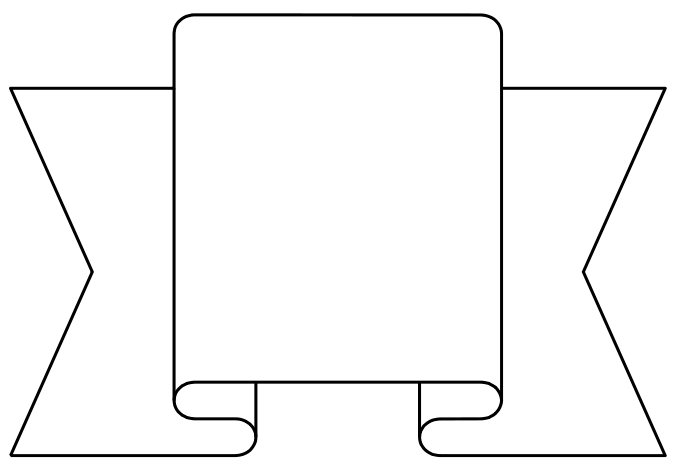
\includegraphics[width=4cm, keepaspectratio]{remarks.png}
			\captionof*{figure}{REMARKS}
		\end{center}
	}

	\vspace{0.5cm}
	supervised by

	\parbox[l]{8cm}{\begin{center}

			SABIHA ANAN\\
\footnotesize{Assistant Professor\\
				Department of CSE, CUET}
		\end{center}
	}
	\parbox[r]{8cm}{\begin{center}

			MD RASHADUR RAHMAN\\
\footnotesize{Lecturer \\
				Department of CSE, CUET}
		\end{center}
	}

	\vfill
\end{titlepage}


\onehalfspacing

\section*{Experiment Name}
Completion of home, signin and signup page  of "SmartHaat" Website
\section*{Objectives}
\begin{itemize}
	\item Designing of home page with footer and search bar etc.
	\item To design login and signup page.
	\item Design the Data Base (making ER Diagram, doing Relational Mapping and Normalization).
\end{itemize}
\section*{Description}
The modified design of home page along with new features are introduced after the last labwork where basic format of home page were developed.
\begin{figure}[H]
	
\includegraphics[keepaspectratio, width=\linewidth ]{coursel1.png}
	\caption{home page carousel}
	\label{coursel1}
\end{figure}
\begin{figure}[]
	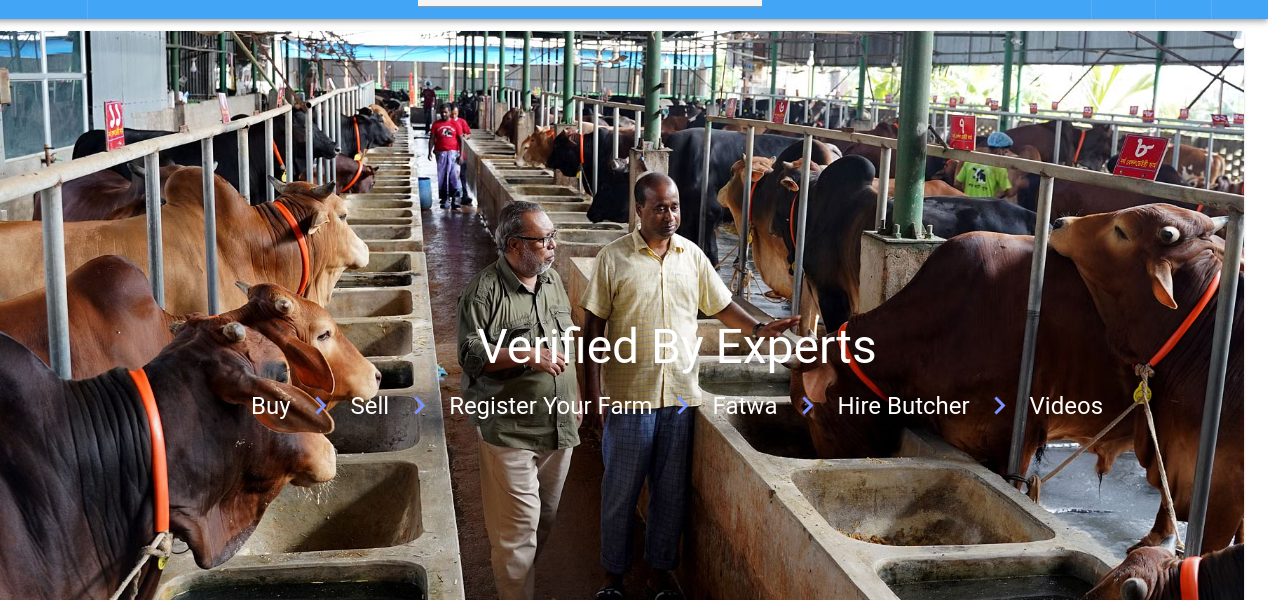
\includegraphics[keepaspectratio, width=\linewidth ]{coursel2.png}
	\caption{home page carousel of experts}
	\label{coursel2}
\end{figure}
The first feature added in the home or main page is the carousel of different links such as,
\begin{itemize}
	\item livestock page
	\item cattle sale for farmars
	\item farms and their products
	\item experts suggession
	\item learn from scholars
	\item upload and register
	\item butcher service
\end{itemize}
From the figure \ref{coursel1} which shows the scholar opinion page and figure \ref{coursel2} shows the verified expertise people are included here as an example.
In the home page the search button is also added for searching items in the webpage.

\begin{figure}[]
	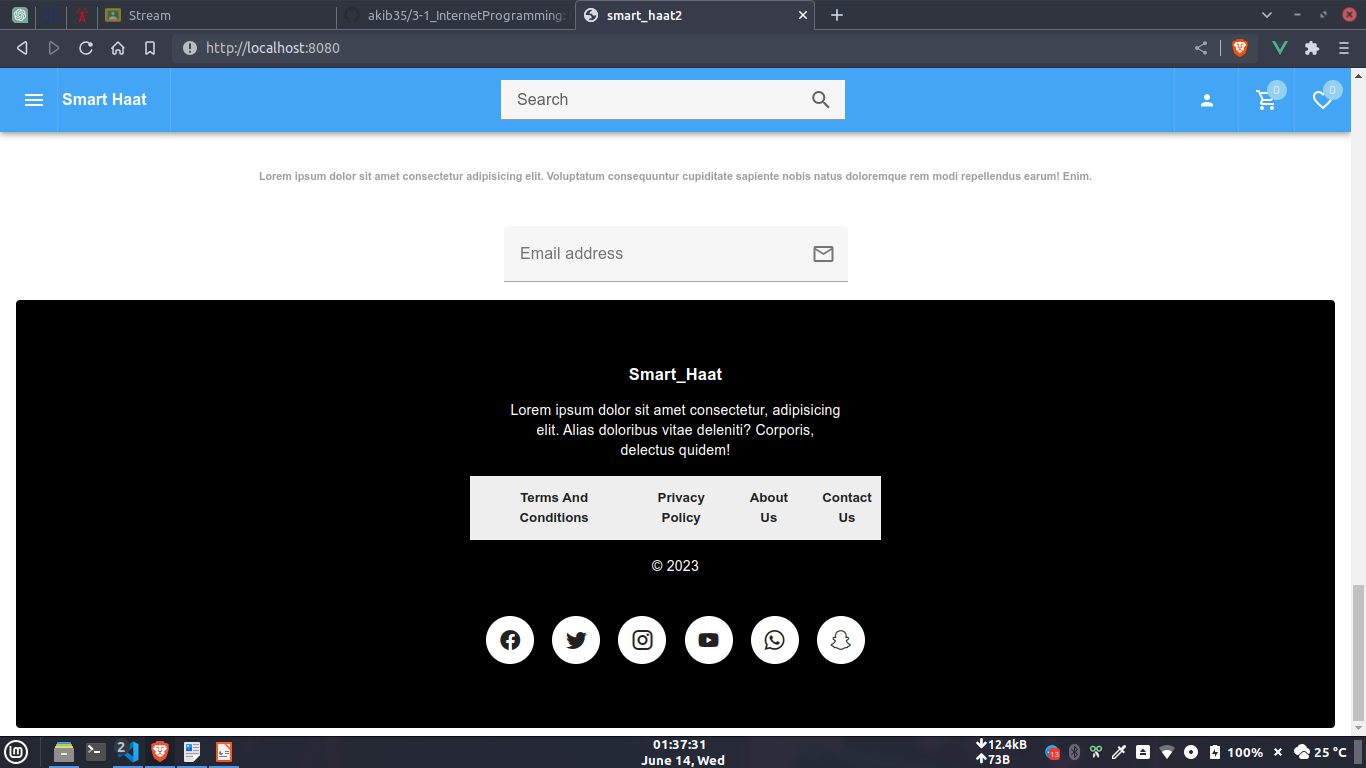
\includegraphics[keepaspectratio, width=\linewidth]{footer.png}
	\caption{home page footer}
	\label{footer}
\end{figure}
Then we improved our home page with suitable footer which is  is added which includes,
\begin{itemize}
	\item email subscription box
	\item social media links
	\item site roadmap links etc.
\end{itemize}
From the figure \ref{footer} the listed items are visible.

\begin{figure}[]
	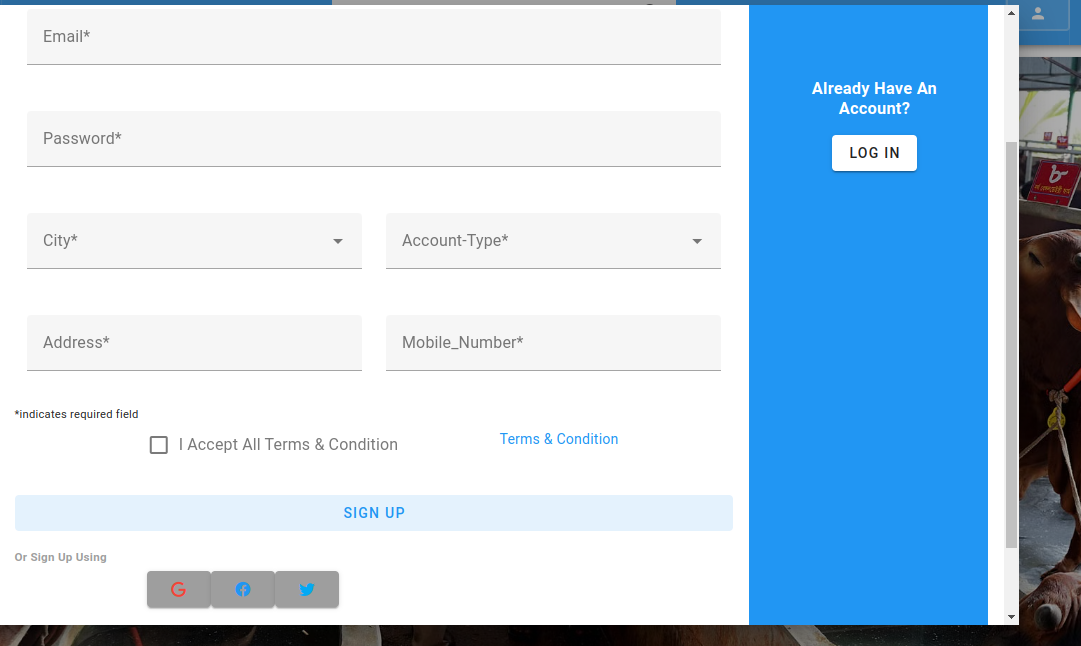
\includegraphics[keepaspectratio, width=\linewidth]{signin.png}
	\caption{login frame}
	\label{login}
	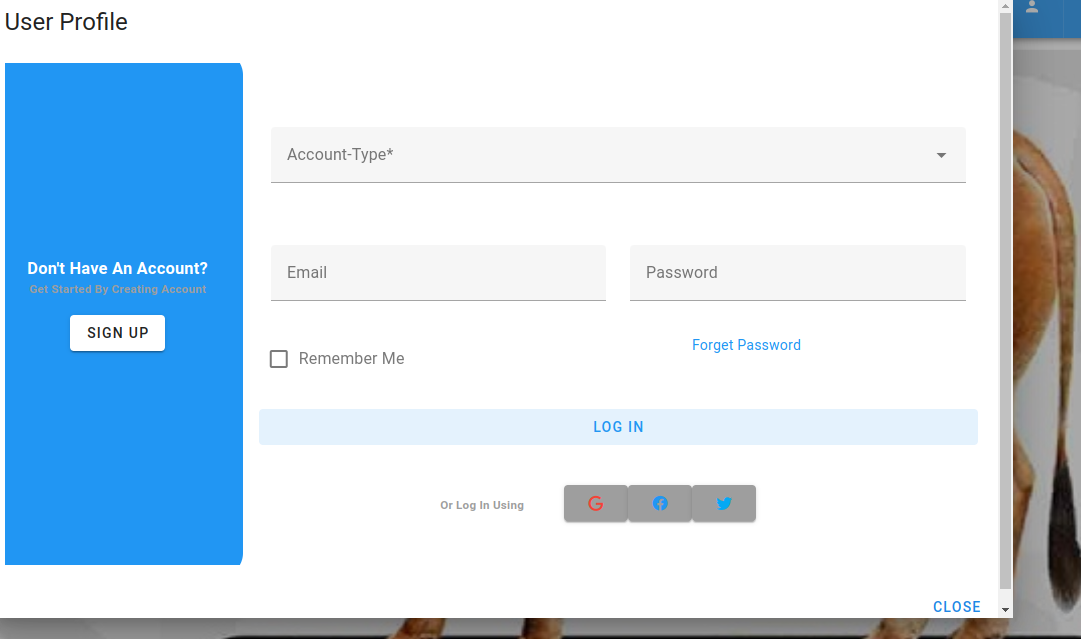
\includegraphics[keepaspectratio , width=\linewidth]{signup.png}
	\caption{signup page}
	\label{signup}
\end{figure}

Furthermore, there are login and signin option shown in figure \ref{login} and figure \ref{signup} where data fields are created for taking data from user and perform the task. There is a close button at the bottom of the page in case we want to exit.

\begin{figure}[H]
	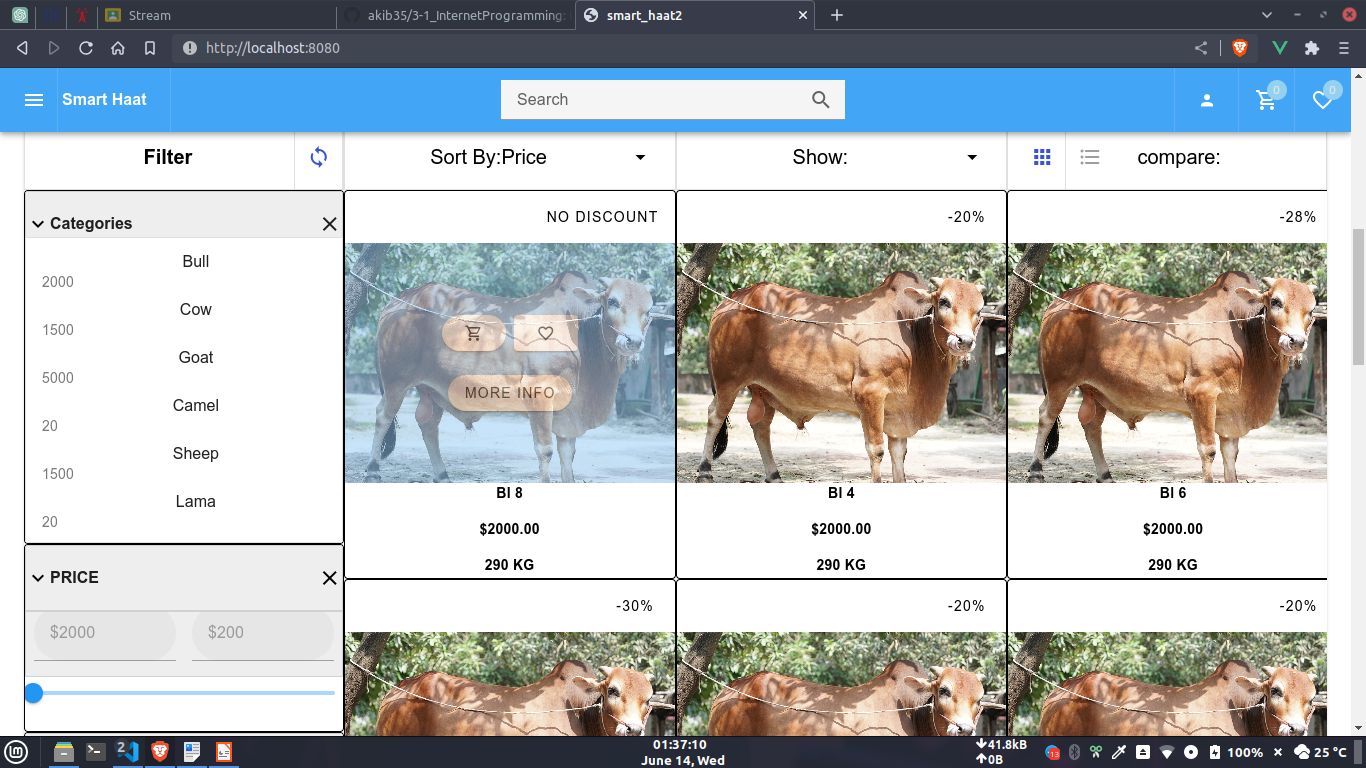
\includegraphics[keepaspectratio, width=\linewidth]{body.png}
	\caption{body section with shaded area and cart button}
	\label{body}
\end{figure}
The middle section of the home page is also improved by using shaded graphics and some buttons such as cart and wishlist.


\begin{figure}
	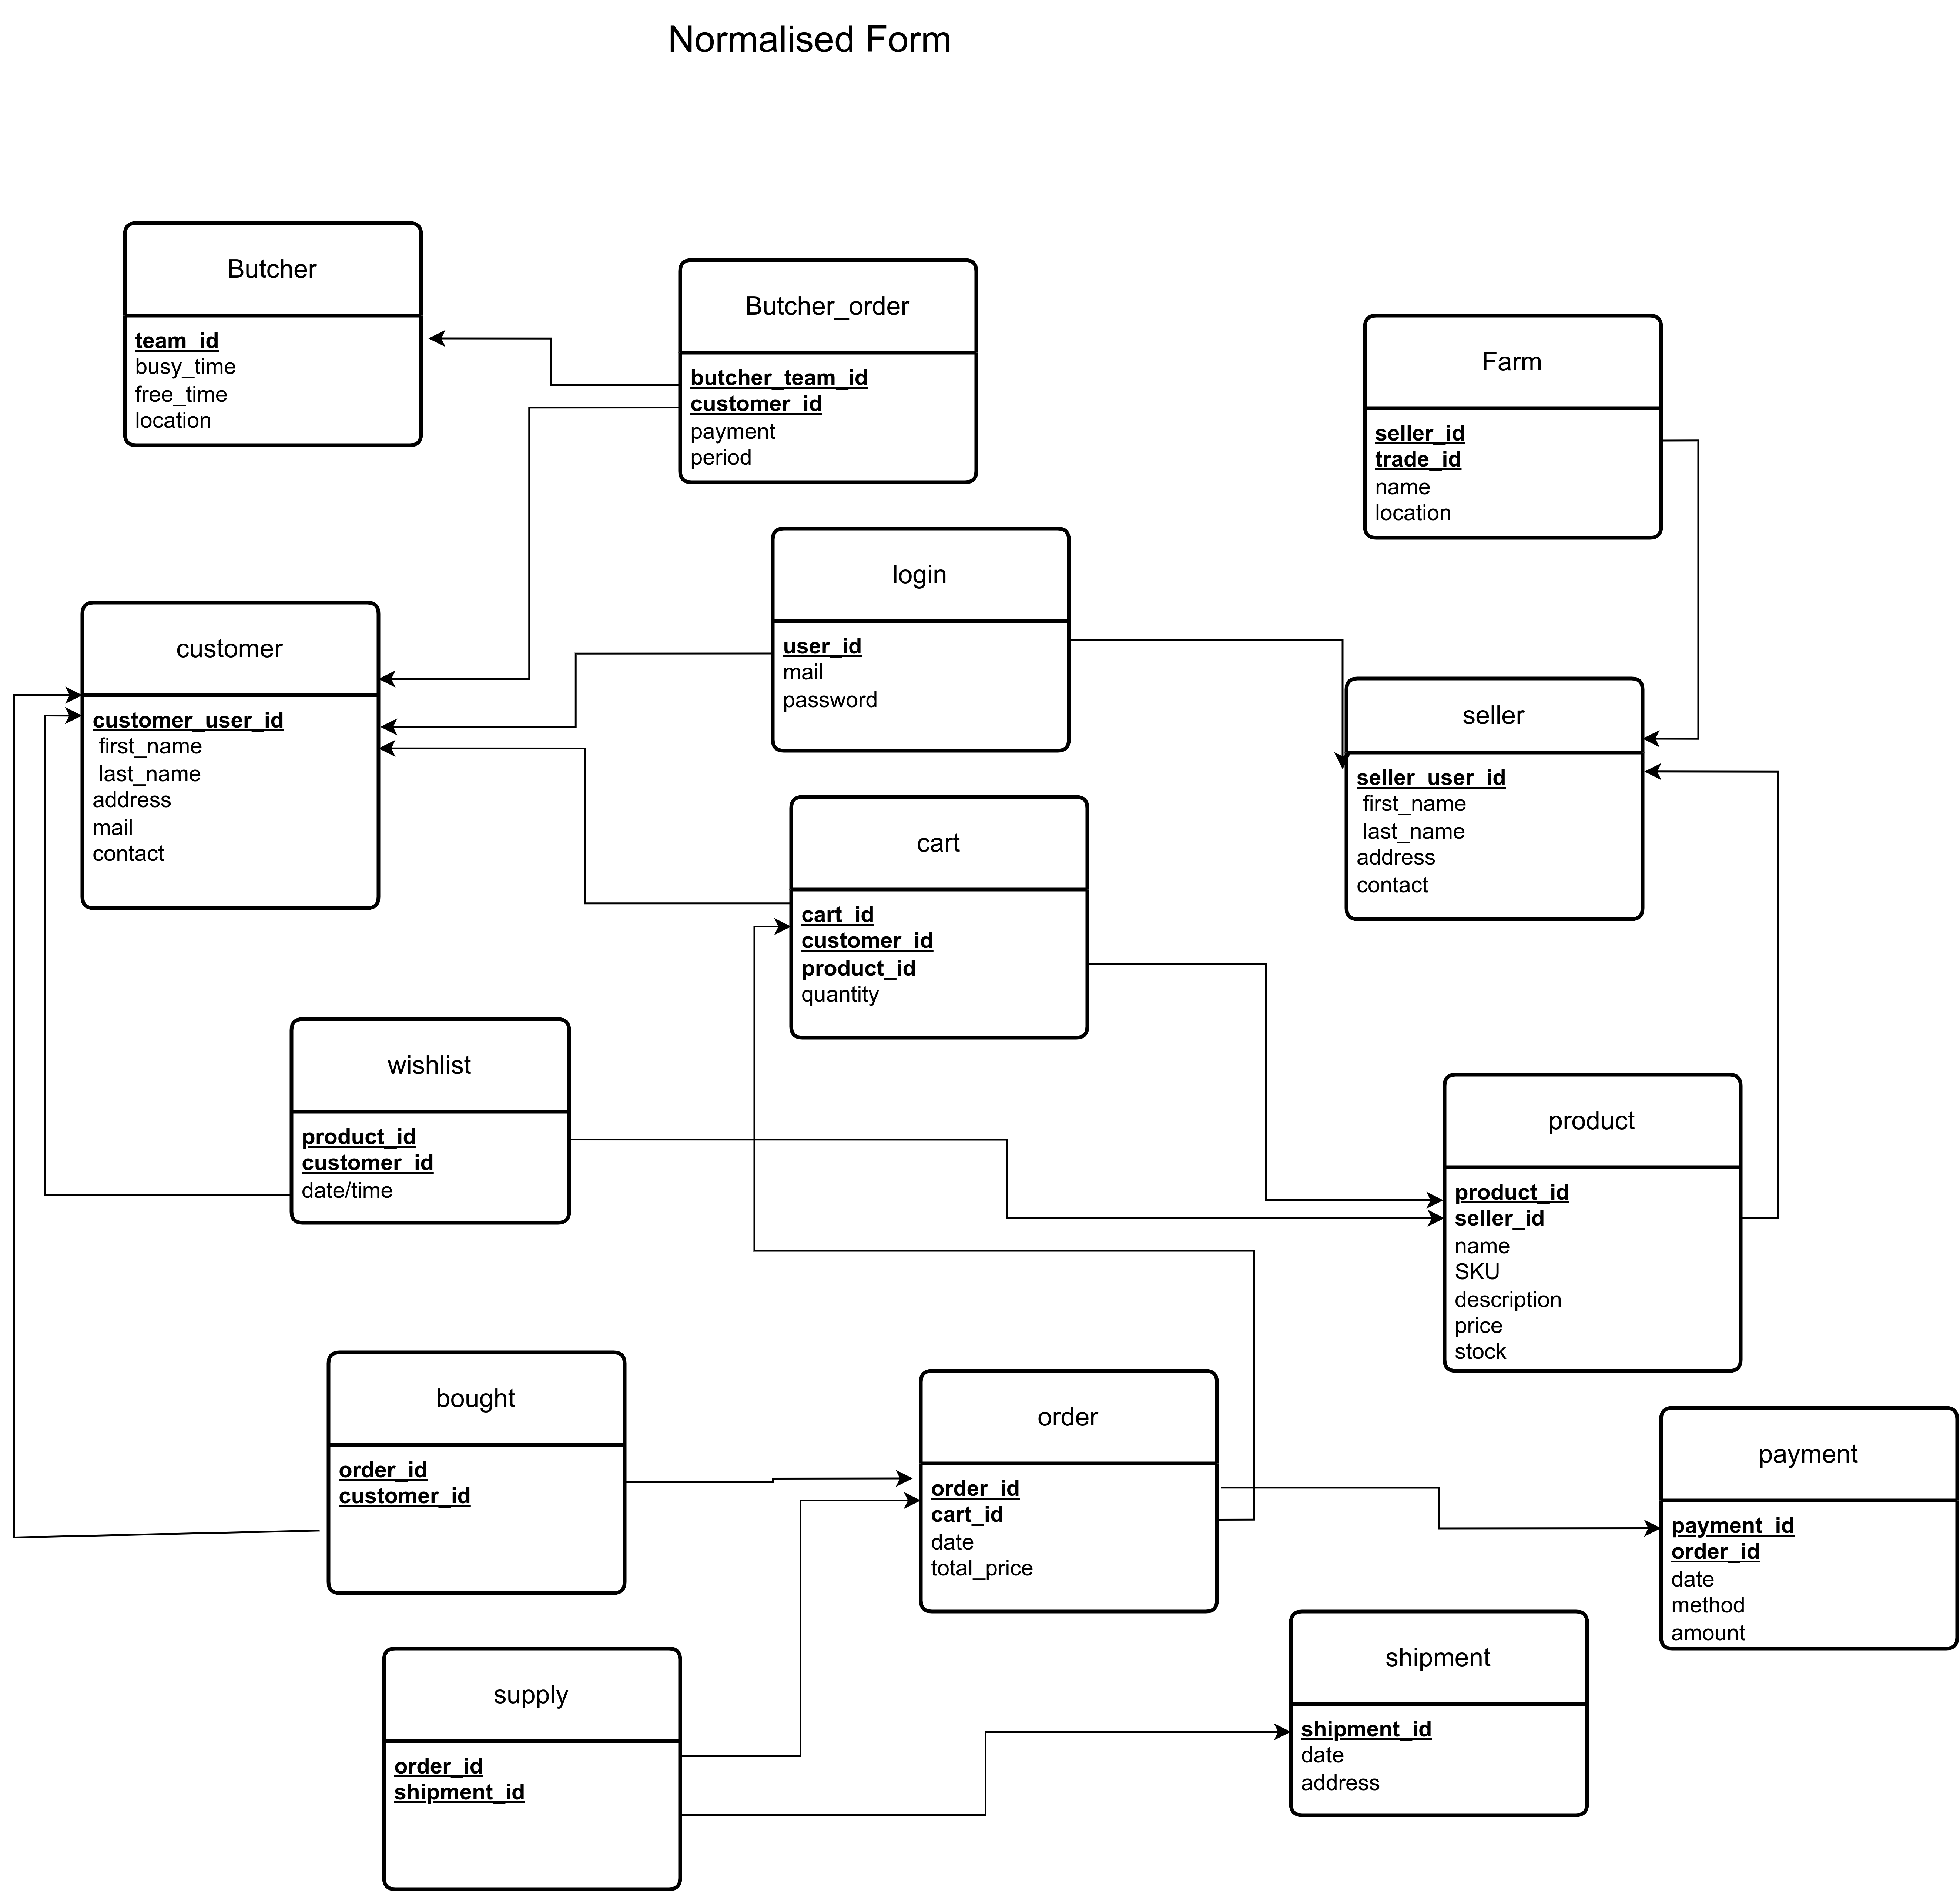
\includegraphics[keepaspectratio, width=\linewidth]{smartHattdbmapping.png}
	\caption{relational mapping of database}
	\label{mapping}
\end{figure}
Finally the relational mapping of our project is shown in figure \ref{mapping}. There are several tables in the diagram such as, 
\begin{itemize}
	\item customer
	\item login
	\item seller
	\item product
	\item butcher
	\item farms
	\item order, etc.
\end{itemize}
 Among these tables there are relation between them which are converted to mapping by transferring the primart key as foreign key etc.

\section*{Development Platfroms}
The frameworks and language platforms we used --
\begin{itemize}
	\item HTML
	\item CSS
	\item JAVASCRIPT
	\item VUE
\end{itemize}

\section*{Conclusion}
In this week we started to devlop our home page with it's funtionalities and features. The header part was improved and footer was added. The login and signup page was introduced. There was an import problem for which we couldn't show the relational mapping last week. So, we included this part here with good quality image resolution.

\end{document}
